% Options for packages loaded elsewhere
\PassOptionsToPackage{unicode}{hyperref}
\PassOptionsToPackage{hyphens}{url}
%
\documentclass[
]{article}
\title{Project}
\author{}
\date{\vspace{-2.5em}}

\usepackage{amsmath,amssymb}
\usepackage{lmodern}
\usepackage{iftex}
\ifPDFTeX
  \usepackage[T1]{fontenc}
  \usepackage[utf8]{inputenc}
  \usepackage{textcomp} % provide euro and other symbols
\else % if luatex or xetex
  \usepackage{unicode-math}
  \defaultfontfeatures{Scale=MatchLowercase}
  \defaultfontfeatures[\rmfamily]{Ligatures=TeX,Scale=1}
\fi
% Use upquote if available, for straight quotes in verbatim environments
\IfFileExists{upquote.sty}{\usepackage{upquote}}{}
\IfFileExists{microtype.sty}{% use microtype if available
  \usepackage[]{microtype}
  \UseMicrotypeSet[protrusion]{basicmath} % disable protrusion for tt fonts
}{}
\makeatletter
\@ifundefined{KOMAClassName}{% if non-KOMA class
  \IfFileExists{parskip.sty}{%
    \usepackage{parskip}
  }{% else
    \setlength{\parindent}{0pt}
    \setlength{\parskip}{6pt plus 2pt minus 1pt}}
}{% if KOMA class
  \KOMAoptions{parskip=half}}
\makeatother
\usepackage{xcolor}
\IfFileExists{xurl.sty}{\usepackage{xurl}}{} % add URL line breaks if available
\IfFileExists{bookmark.sty}{\usepackage{bookmark}}{\usepackage{hyperref}}
\hypersetup{
  pdftitle={Project},
  hidelinks,
  pdfcreator={LaTeX via pandoc}}
\urlstyle{same} % disable monospaced font for URLs
\usepackage[margin=1in]{geometry}
\usepackage{color}
\usepackage{fancyvrb}
\newcommand{\VerbBar}{|}
\newcommand{\VERB}{\Verb[commandchars=\\\{\}]}
\DefineVerbatimEnvironment{Highlighting}{Verbatim}{commandchars=\\\{\}}
% Add ',fontsize=\small' for more characters per line
\usepackage{framed}
\definecolor{shadecolor}{RGB}{248,248,248}
\newenvironment{Shaded}{\begin{snugshade}}{\end{snugshade}}
\newcommand{\AlertTok}[1]{\textcolor[rgb]{0.94,0.16,0.16}{#1}}
\newcommand{\AnnotationTok}[1]{\textcolor[rgb]{0.56,0.35,0.01}{\textbf{\textit{#1}}}}
\newcommand{\AttributeTok}[1]{\textcolor[rgb]{0.77,0.63,0.00}{#1}}
\newcommand{\BaseNTok}[1]{\textcolor[rgb]{0.00,0.00,0.81}{#1}}
\newcommand{\BuiltInTok}[1]{#1}
\newcommand{\CharTok}[1]{\textcolor[rgb]{0.31,0.60,0.02}{#1}}
\newcommand{\CommentTok}[1]{\textcolor[rgb]{0.56,0.35,0.01}{\textit{#1}}}
\newcommand{\CommentVarTok}[1]{\textcolor[rgb]{0.56,0.35,0.01}{\textbf{\textit{#1}}}}
\newcommand{\ConstantTok}[1]{\textcolor[rgb]{0.00,0.00,0.00}{#1}}
\newcommand{\ControlFlowTok}[1]{\textcolor[rgb]{0.13,0.29,0.53}{\textbf{#1}}}
\newcommand{\DataTypeTok}[1]{\textcolor[rgb]{0.13,0.29,0.53}{#1}}
\newcommand{\DecValTok}[1]{\textcolor[rgb]{0.00,0.00,0.81}{#1}}
\newcommand{\DocumentationTok}[1]{\textcolor[rgb]{0.56,0.35,0.01}{\textbf{\textit{#1}}}}
\newcommand{\ErrorTok}[1]{\textcolor[rgb]{0.64,0.00,0.00}{\textbf{#1}}}
\newcommand{\ExtensionTok}[1]{#1}
\newcommand{\FloatTok}[1]{\textcolor[rgb]{0.00,0.00,0.81}{#1}}
\newcommand{\FunctionTok}[1]{\textcolor[rgb]{0.00,0.00,0.00}{#1}}
\newcommand{\ImportTok}[1]{#1}
\newcommand{\InformationTok}[1]{\textcolor[rgb]{0.56,0.35,0.01}{\textbf{\textit{#1}}}}
\newcommand{\KeywordTok}[1]{\textcolor[rgb]{0.13,0.29,0.53}{\textbf{#1}}}
\newcommand{\NormalTok}[1]{#1}
\newcommand{\OperatorTok}[1]{\textcolor[rgb]{0.81,0.36,0.00}{\textbf{#1}}}
\newcommand{\OtherTok}[1]{\textcolor[rgb]{0.56,0.35,0.01}{#1}}
\newcommand{\PreprocessorTok}[1]{\textcolor[rgb]{0.56,0.35,0.01}{\textit{#1}}}
\newcommand{\RegionMarkerTok}[1]{#1}
\newcommand{\SpecialCharTok}[1]{\textcolor[rgb]{0.00,0.00,0.00}{#1}}
\newcommand{\SpecialStringTok}[1]{\textcolor[rgb]{0.31,0.60,0.02}{#1}}
\newcommand{\StringTok}[1]{\textcolor[rgb]{0.31,0.60,0.02}{#1}}
\newcommand{\VariableTok}[1]{\textcolor[rgb]{0.00,0.00,0.00}{#1}}
\newcommand{\VerbatimStringTok}[1]{\textcolor[rgb]{0.31,0.60,0.02}{#1}}
\newcommand{\WarningTok}[1]{\textcolor[rgb]{0.56,0.35,0.01}{\textbf{\textit{#1}}}}
\usepackage{graphicx}
\makeatletter
\def\maxwidth{\ifdim\Gin@nat@width>\linewidth\linewidth\else\Gin@nat@width\fi}
\def\maxheight{\ifdim\Gin@nat@height>\textheight\textheight\else\Gin@nat@height\fi}
\makeatother
% Scale images if necessary, so that they will not overflow the page
% margins by default, and it is still possible to overwrite the defaults
% using explicit options in \includegraphics[width, height, ...]{}
\setkeys{Gin}{width=\maxwidth,height=\maxheight,keepaspectratio}
% Set default figure placement to htbp
\makeatletter
\def\fps@figure{htbp}
\makeatother
\setlength{\emergencystretch}{3em} % prevent overfull lines
\providecommand{\tightlist}{%
  \setlength{\itemsep}{0pt}\setlength{\parskip}{0pt}}
\setcounter{secnumdepth}{-\maxdimen} % remove section numbering
\ifLuaTeX
  \usepackage{selnolig}  % disable illegal ligatures
\fi

\begin{document}
\maketitle

\hypertarget{library-imports}{%
\subsection{Library Imports}\label{library-imports}}

\begin{Shaded}
\begin{Highlighting}[]
\CommentTok{\#install.packages("adegenet")}
\FunctionTok{library}\NormalTok{(adegenet)}
\FunctionTok{library}\NormalTok{(ggplot2)}
\FunctionTok{library}\NormalTok{(tidyverse)}
\FunctionTok{library}\NormalTok{(here)}
\FunctionTok{library}\NormalTok{(janitor)}
\end{Highlighting}
\end{Shaded}

\hypertarget{import-dataset}{%
\subsection{Import Dataset}\label{import-dataset}}

\begin{Shaded}
\begin{Highlighting}[]
\NormalTok{week\_gene }\OtherTok{\textless{}{-}} \FunctionTok{read.csv}\NormalTok{(}\StringTok{"data/weeks\_genotypes.csv"}\NormalTok{)}
\FunctionTok{head}\NormalTok{(week\_gene)}
\end{Highlighting}
\end{Shaded}

\begin{verbatim}
##   ID      Pop Year    LOC1    LOC2    LOC3    LOC4    LOC5    LOC6    LOC7
## 1  1 MtBuller 2010 311/311 245/249 303/303 195/201 218/218 211/211 321/321
## 2  2 MtBuller 2010 311/311 245/249 303/303 195/201 218/218 211/211 321/321
## 3  3 MtBuller 2010 311/311 245/249 303/303   NA/NA 218/218 211/211 321/321
## 4  4 MtBuller 2010 311/311 249/249 303/303 195/195 218/218 211/211 321/321
## 5  5 MtBuller 2010 309/311 249/249 303/303 195/201 218/218 211/211 321/321
## 6  6 MtBuller 2010 309/311   NA/NA 303/303 201/201 218/218 211/211 321/321
##      LOC8    LOC9   LOC10   LOC11   LOC12   LOC13   LOC14   LOC15   LOC16
## 1 240/240 157/157 113/113 178/178 125/125 309/318 119/119 144/146 214/214
## 2 240/240 157/157 113/113 178/178 125/125 309/309 119/148 144/146 214/214
## 3 240/240 157/157 113/113 178/178 125/125 309/309 119/119 144/144 214/216
## 4 240/240 157/157 113/113 178/178 125/125 309/309 119/119 144/146 214/214
## 5 240/240 157/157 113/115 178/178 125/125 309/318 148/148 144/146 216/216
## 6 240/240 157/157 113/115 178/178 125/125 309/318 119/148 144/144 214/214
##     LOC17   LOC18   LOC19   LOC20   LOC21   LOC22   LOC23   LOC24
## 1 241/241 160/160 150/150 117/117 141/141 137/137 157/157 177/177
## 2 241/241 160/160 150/150 117/117 141/141 137/137 157/157 177/177
## 3 241/241 160/160 150/150 117/117 141/141 137/137 157/157 177/177
## 4 241/241 160/160 150/150 117/117 141/141 137/137 157/157 177/177
## 5 241/241 160/160 150/150 117/117 141/141 137/141 157/157 177/177
## 6 241/241 160/160 150/150 117/117 141/141 137/137 157/157 177/177
\end{verbatim}

\hypertarget{determine-heterozygosity}{%
\subsection{Determine Heterozygosity}\label{determine-heterozygosity}}

\begin{Shaded}
\begin{Highlighting}[]
\NormalTok{alleles }\OtherTok{\textless{}{-}}\NormalTok{ week\_gene[,}\DecValTok{4}\SpecialCharTok{:}\FunctionTok{ncol}\NormalTok{(week\_gene)]}
\NormalTok{genind\_alleles }\OtherTok{\textless{}{-}} \FunctionTok{df2genind}\NormalTok{(alleles,}\AttributeTok{sep=}\StringTok{"/"}\NormalTok{,}\AttributeTok{NA.char=}\StringTok{"NA/NA"}\NormalTok{)}
\NormalTok{heterozygosity\_results }\OtherTok{\textless{}{-}} \FunctionTok{summary}\NormalTok{(genind\_alleles)}
\NormalTok{heterozygosity\_results}
\end{Highlighting}
\end{Shaded}

\begin{verbatim}
## 
## // Number of individuals: 524
## // Group sizes: 524
## // Number of alleles per locus: 5 5 10 7 8 3 7 16 3 11 10 2 6 10 5 2 10 2 5 3 2 10 9 4
## // Number of alleles per group: 155
## // Percentage of missing data: 1.03 %
## // Observed heterozygosity: 0.12 0.68 0.29 0.6 0.48 0.3 0.36 0.38 0.35 0.64 0.43 0.22 0.54 0.6 0.5 0.21 0.38 0.25 0.25 0.17 0.17 0.39 0.26 0.25
## // Expected heterozygosity: 0.12 0.64 0.36 0.7 0.58 0.32 0.5 0.56 0.51 0.74 0.56 0.45 0.64 0.61 0.63 0.25 0.44 0.46 0.29 0.19 0.35 0.49 0.33 0.38
\end{verbatim}

\hypertarget{heterozygosity-by-population}{%
\subsection{Heterozygosity by
Population}\label{heterozygosity-by-population}}

\begin{Shaded}
\begin{Highlighting}[]
\NormalTok{pop\_geind\_alleles }\OtherTok{\textless{}{-}} \FunctionTok{seppop}\NormalTok{(}\FunctionTok{df2genind}\NormalTok{(alleles,}\AttributeTok{sep=}\StringTok{"/"}\NormalTok{,}\AttributeTok{NA.char=}\StringTok{"NA/NA"}\NormalTok{, }\AttributeTok{pop=}\NormalTok{week\_gene}\SpecialCharTok{$}\NormalTok{Pop))}
\NormalTok{pop\_geind\_alleles}
\end{Highlighting}
\end{Shaded}

\begin{verbatim}
## $MtBuller
## /// GENIND OBJECT /////////
## 
##  // 420 individuals; 24 loci; 155 alleles; size: 316.4 Kb
## 
##  // Basic content
##    @tab:  420 x 155 matrix of allele counts
##    @loc.n.all: number of alleles per locus (range: 2-16)
##    @loc.fac: locus factor for the 155 columns of @tab
##    @all.names: list of allele names for each locus
##    @ploidy: ploidy of each individual  (range: 2-2)
##    @type:  codom
##    @call: .local(x = x, i = i, j = j, pop = ..1, treatOther = ..2, quiet = ..3, 
##     drop = drop)
## 
##  // Optional content
##    @pop: population of each individual (group size range: 420-420)
## 
## $MtHigginbotham
## /// GENIND OBJECT /////////
## 
##  // 104 individuals; 24 loci; 155 alleles; size: 102.9 Kb
## 
##  // Basic content
##    @tab:  104 x 155 matrix of allele counts
##    @loc.n.all: number of alleles per locus (range: 2-16)
##    @loc.fac: locus factor for the 155 columns of @tab
##    @all.names: list of allele names for each locus
##    @ploidy: ploidy of each individual  (range: 2-2)
##    @type:  codom
##    @call: .local(x = x, i = i, j = j, pop = ..1, treatOther = ..2, quiet = ..3, 
##     drop = drop)
## 
##  // Optional content
##    @pop: population of each individual (group size range: 104-104)
\end{verbatim}

\hypertarget{group-by-population}{%
\subsection{Group by Population}\label{group-by-population}}

\begin{Shaded}
\begin{Highlighting}[]
\NormalTok{MtBuller }\OtherTok{\textless{}{-}} \FunctionTok{summary}\NormalTok{(pop\_geind\_alleles}\SpecialCharTok{$}\NormalTok{MtBuller)}
\NormalTok{MtHiggenbotham }\OtherTok{\textless{}{-}} \FunctionTok{summary}\NormalTok{(pop\_geind\_alleles}\SpecialCharTok{$}\NormalTok{MtHigginbotham)}
\NormalTok{MtBuller}
\end{Highlighting}
\end{Shaded}

\begin{verbatim}
## 
## // Number of individuals: 420
## // Group sizes: 420
## // Number of alleles per locus: 4 4 4 7 7 2 6 10 3 7 8 2 5 5 5 2 6 2 4 3 2 9 5 4
## // Number of alleles per group: 116
## // Percentage of missing data: 0.64 %
## // Observed heterozygosity: 0.12 0.65 0.21 0.56 0.39 0.26 0.29 0.33 0.34 0.62 0.33 0.27 0.51 0.58 0.49 0.26 0.26 0.31 0.17 0.15 0.14 0.31 0.16 0.15
## // Expected heterozygosity: 0.11 0.61 0.23 0.61 0.4 0.25 0.29 0.36 0.34 0.64 0.34 0.3 0.51 0.57 0.51 0.3 0.26 0.33 0.16 0.18 0.16 0.35 0.16 0.17
\end{verbatim}

\hypertarget{create-dataframes-for-comparing-observed-and-expected}{%
\subsection{Create dataframes for comparing observed and
expected}\label{create-dataframes-for-comparing-observed-and-expected}}

\begin{Shaded}
\begin{Highlighting}[]
\NormalTok{MtBullerDf }\OtherTok{\textless{}{-}} \FunctionTok{data.frame}\NormalTok{(}\FunctionTok{unlist}\NormalTok{(MtBuller}\SpecialCharTok{$}\NormalTok{Hobs), }\FunctionTok{unlist}\NormalTok{(MtBuller}\SpecialCharTok{$}\NormalTok{Hexp))}
\FunctionTok{names}\NormalTok{(MtBullerDf) }\OtherTok{\textless{}{-}} \FunctionTok{c}\NormalTok{(}\StringTok{"Hobs"}\NormalTok{, }\StringTok{"Hexp"}\NormalTok{)}
\NormalTok{MtHiggenbothamDf }\OtherTok{\textless{}{-}} \FunctionTok{data.frame}\NormalTok{(}\FunctionTok{unlist}\NormalTok{(MtHiggenbotham}\SpecialCharTok{$}\NormalTok{Hobs), }\FunctionTok{unlist}\NormalTok{(MtHiggenbotham}\SpecialCharTok{$}\NormalTok{Hexp))}
\FunctionTok{names}\NormalTok{(MtHiggenbothamDf) }\OtherTok{\textless{}{-}} \FunctionTok{c}\NormalTok{(}\StringTok{"Hobs"}\NormalTok{, }\StringTok{"Hexp"}\NormalTok{)}
\FunctionTok{head}\NormalTok{(MtBullerDf)}
\end{Highlighting}
\end{Shaded}

\begin{verbatim}
##           Hobs      Hexp
## LOC1 0.1196172 0.1129982
## LOC2 0.6526055 0.6064596
## LOC3 0.2120482 0.2329279
## LOC4 0.5649038 0.6085111
## LOC5 0.3937947 0.4022334
## LOC6 0.2583732 0.2458735
\end{verbatim}

\hypertarget{dataframes-pivoted-on-observation-type}{%
\subsection{Dataframes Pivoted on Observation
Type}\label{dataframes-pivoted-on-observation-type}}

\begin{Shaded}
\begin{Highlighting}[]
\NormalTok{category }\OtherTok{\textless{}{-}} \FunctionTok{rep}\NormalTok{(}\FunctionTok{c}\NormalTok{(}\StringTok{"Observed"}\NormalTok{, }\StringTok{"Expected"}\NormalTok{), }\AttributeTok{each=}\FunctionTok{length}\NormalTok{(MtBullerDf}\SpecialCharTok{$}\NormalTok{Hobs))}
\NormalTok{MtBullerPivot }\OtherTok{\textless{}{-}} \FunctionTok{data.frame}\NormalTok{(}\FunctionTok{c}\NormalTok{(}\FunctionTok{seq}\NormalTok{(}\DecValTok{1}\NormalTok{, }\DecValTok{24}\NormalTok{, }\DecValTok{1}\NormalTok{), }\FunctionTok{seq}\NormalTok{(}\DecValTok{1}\NormalTok{, }\DecValTok{24}\NormalTok{, }\DecValTok{1}\NormalTok{)), }\FunctionTok{c}\NormalTok{(MtBullerDf}\SpecialCharTok{$}\NormalTok{Hobs, MtBullerDf}\SpecialCharTok{$}\NormalTok{Hexp), category)}
\NormalTok{MtHiggenbothamPivot }\OtherTok{\textless{}{-}} \FunctionTok{data.frame}\NormalTok{(}\FunctionTok{c}\NormalTok{(}\FunctionTok{seq}\NormalTok{(}\DecValTok{1}\NormalTok{, }\DecValTok{24}\NormalTok{, }\DecValTok{1}\NormalTok{), }\FunctionTok{seq}\NormalTok{(}\DecValTok{1}\NormalTok{, }\DecValTok{24}\NormalTok{, }\DecValTok{1}\NormalTok{)), }\FunctionTok{c}\NormalTok{(MtHiggenbothamDf}\SpecialCharTok{$}\NormalTok{Hobs, MtHiggenbothamDf}\SpecialCharTok{$}\NormalTok{Hexp), category)}
\FunctionTok{names}\NormalTok{(MtBullerPivot) }\OtherTok{\textless{}{-}} \FunctionTok{c}\NormalTok{(}\StringTok{"Location"}\NormalTok{, }\StringTok{"Heterozygosity"}\NormalTok{, }\StringTok{"Type"}\NormalTok{)}
\FunctionTok{names}\NormalTok{(MtHiggenbothamPivot) }\OtherTok{\textless{}{-}} \FunctionTok{c}\NormalTok{(}\StringTok{"Location"}\NormalTok{, }\StringTok{"Heterozygosity"}\NormalTok{, }\StringTok{"Type"}\NormalTok{)}
\FunctionTok{head}\NormalTok{(MtBullerPivot)}
\end{Highlighting}
\end{Shaded}

\begin{verbatim}
##   Location Heterozygosity     Type
## 1        1      0.1196172 Observed
## 2        2      0.6526055 Observed
## 3        3      0.2120482 Observed
## 4        4      0.5649038 Observed
## 5        5      0.3937947 Observed
## 6        6      0.2583732 Observed
\end{verbatim}

\hypertarget{boxplot-comparison-mtbuller}{%
\subsection{Boxplot Comparison
MtBuller}\label{boxplot-comparison-mtbuller}}

\begin{Shaded}
\begin{Highlighting}[]
\NormalTok{MtBullerPivot }\SpecialCharTok{\%\textgreater{}\%} 
  \FunctionTok{ggplot}\NormalTok{(}\FunctionTok{aes}\NormalTok{(}\AttributeTok{x=}\NormalTok{Type, }\AttributeTok{y=}\NormalTok{Heterozygosity)) }\SpecialCharTok{+} \FunctionTok{geom\_boxplot}\NormalTok{(}\AttributeTok{na.rm=}\NormalTok{T) }\SpecialCharTok{+} \FunctionTok{coord\_flip}\NormalTok{()}
\end{Highlighting}
\end{Shaded}

\includegraphics{Report_files/figure-latex/boxplotbuller-1.pdf}

\hypertarget{boxplot-comparison-mthiggenbotham}{%
\subsection{Boxplot Comparison
MtHiggenbotham}\label{boxplot-comparison-mthiggenbotham}}

\begin{Shaded}
\begin{Highlighting}[]
\NormalTok{MtHiggenbothamPivot }\SpecialCharTok{\%\textgreater{}\%} 
  \FunctionTok{ggplot}\NormalTok{(}\FunctionTok{aes}\NormalTok{(}\AttributeTok{x=}\NormalTok{Type, }\AttributeTok{y=}\NormalTok{Heterozygosity)) }\SpecialCharTok{+} \FunctionTok{geom\_boxplot}\NormalTok{(}\AttributeTok{na.rm=}\NormalTok{T) }\SpecialCharTok{+} \FunctionTok{coord\_flip}\NormalTok{()}
\end{Highlighting}
\end{Shaded}

\includegraphics{Report_files/figure-latex/boxplothiggenbotham-1.pdf}

\hypertarget{barplot-comparison-mtbuller}{%
\subsection{Barplot Comparison
MtBuller}\label{barplot-comparison-mtbuller}}

\begin{Shaded}
\begin{Highlighting}[]
\NormalTok{MtBullerPivot }\SpecialCharTok{\%\textgreater{}\%}
  \FunctionTok{ggplot}\NormalTok{(}\FunctionTok{aes}\NormalTok{(}\AttributeTok{x=}\NormalTok{Location, }\AttributeTok{y=}\NormalTok{Heterozygosity, }\AttributeTok{fill=}\NormalTok{Type)) }\SpecialCharTok{+} \FunctionTok{geom\_bar}\NormalTok{(}\AttributeTok{stat=}\StringTok{"identity"}\NormalTok{, }\AttributeTok{position =} \StringTok{"identity"}\NormalTok{, }\AttributeTok{alpha=}\NormalTok{.}\DecValTok{3}\NormalTok{, }\AttributeTok{na.rm=}\NormalTok{T)}
\end{Highlighting}
\end{Shaded}

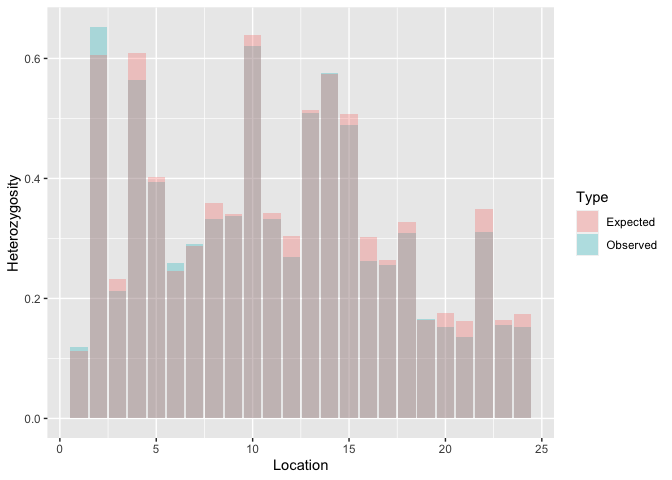
\includegraphics{Report_files/figure-latex/barplotbuller-1.pdf}

\hypertarget{barplot-comparison-mthiggenbotham}{%
\subsection{Barplot Comparison
MtHiggenbotham}\label{barplot-comparison-mthiggenbotham}}

\begin{Shaded}
\begin{Highlighting}[]
\NormalTok{MtHiggenbothamPivot }\SpecialCharTok{\%\textgreater{}\%}
  \FunctionTok{ggplot}\NormalTok{(}\FunctionTok{aes}\NormalTok{(}\AttributeTok{x=}\NormalTok{Location, }\AttributeTok{y=}\NormalTok{Heterozygosity, }\AttributeTok{fill=}\NormalTok{Type)) }\SpecialCharTok{+} \FunctionTok{geom\_bar}\NormalTok{(}\AttributeTok{stat=}\StringTok{"identity"}\NormalTok{, }\AttributeTok{position =} \StringTok{"identity"}\NormalTok{, }\AttributeTok{alpha=}\NormalTok{.}\DecValTok{3}\NormalTok{, }\AttributeTok{na.rm=}\NormalTok{T)}
\end{Highlighting}
\end{Shaded}

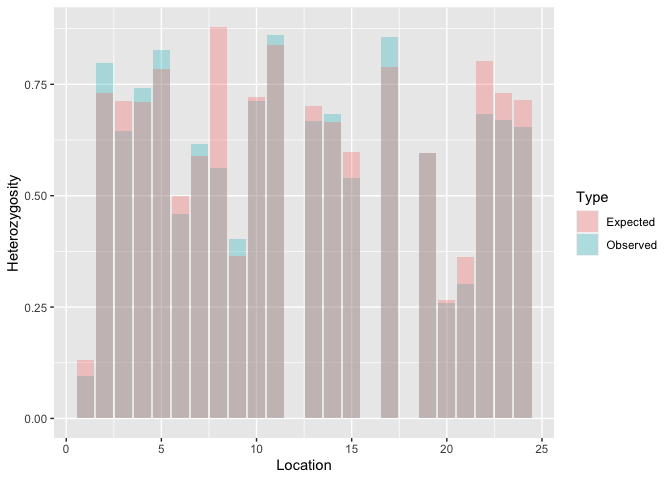
\includegraphics{Report_files/figure-latex/barplothiggenbotham-1.pdf}

\hypertarget{scatterplot-comparison-of-observed-between-mtbuller-and-mthiggenbotham}{%
\subsection{Scatterplot Comparison of Observed between MtBuller and
MtHiggenbotham}\label{scatterplot-comparison-of-observed-between-mtbuller-and-mthiggenbotham}}

\begin{Shaded}
\begin{Highlighting}[]
\NormalTok{combindedPop }\OtherTok{\textless{}{-}} \FunctionTok{rbind}\NormalTok{(MtBullerDf, MtHiggenbothamDf)}
\NormalTok{combindedPop}\SpecialCharTok{$}\NormalTok{Population }\OtherTok{\textless{}{-}} \FunctionTok{rep}\NormalTok{(}\FunctionTok{c}\NormalTok{(}\StringTok{"MtBuller"}\NormalTok{, }\StringTok{"MtHiggenbotham"}\NormalTok{), }\AttributeTok{each=}\DecValTok{24}\NormalTok{)}
\NormalTok{combindedPop}\SpecialCharTok{$}\NormalTok{Location }\OtherTok{\textless{}{-}} \FunctionTok{c}\NormalTok{(}\FunctionTok{seq}\NormalTok{(}\DecValTok{1}\NormalTok{, }\DecValTok{24}\NormalTok{, }\DecValTok{1}\NormalTok{), }\FunctionTok{seq}\NormalTok{(}\DecValTok{1}\NormalTok{, }\DecValTok{24}\NormalTok{, }\DecValTok{1}\NormalTok{))}
\NormalTok{combindedPop }\SpecialCharTok{\%\textgreater{}\%} 
  \FunctionTok{ggplot}\NormalTok{(}\FunctionTok{aes}\NormalTok{(}\AttributeTok{x=}\NormalTok{Location, }\AttributeTok{y=}\NormalTok{Hobs, }\AttributeTok{color=}\NormalTok{Population)) }\SpecialCharTok{+} \FunctionTok{geom\_point}\NormalTok{()}
\end{Highlighting}
\end{Shaded}

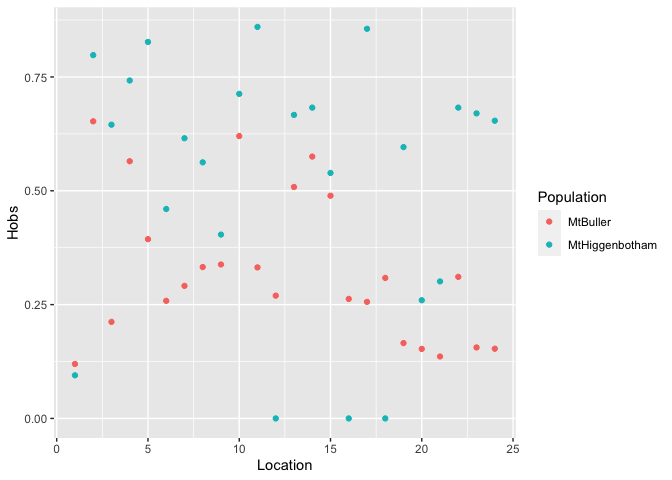
\includegraphics{Report_files/figure-latex/scatterobs-1.pdf}

\hypertarget{scatterplot-comparison-of-expected-between-mtbuller-and-mthiggenbotham}{%
\subsection{Scatterplot Comparison of Expected between MtBuller and
MtHiggenbotham}\label{scatterplot-comparison-of-expected-between-mtbuller-and-mthiggenbotham}}

\begin{Shaded}
\begin{Highlighting}[]
\NormalTok{combindedPop }\SpecialCharTok{\%\textgreater{}\%} 
  \FunctionTok{ggplot}\NormalTok{(}\FunctionTok{aes}\NormalTok{(}\AttributeTok{x=}\NormalTok{Location, }\AttributeTok{y=}\NormalTok{Hexp, }\AttributeTok{color=}\NormalTok{Population)) }\SpecialCharTok{+} \FunctionTok{geom\_point}\NormalTok{()}
\end{Highlighting}
\end{Shaded}

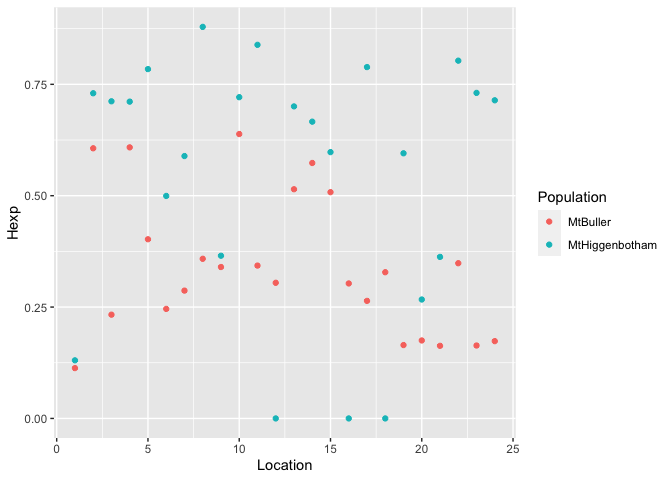
\includegraphics{Report_files/figure-latex/scatterexp-1.pdf}

\end{document}
